% Waves Program Master Degree Template
% Author: Viktoriia Boichenko
% vik.boichenko@gmail.com
\documentclass[a4paper,11pt]{article}

% \usepackage[utf8]{inputenc}
\usepackage{graphicx}
\graphicspath{ figures/ }

% Language setting
\usepackage[english]{babel}
\usepackage{fontspec}
% \setmainfont{Courier New}
% Set page size and margins
\usepackage[letterpaper,top=2.54cm,bottom=2.54cm,left=2.85cm,right=2.85cm,marginparwidth=1.75cm]{geometry}

% Set spacing between lines and sections
\usepackage{titlesec}
\titlespacing*{\section}{0pt}{32pt}{20pt}
\titlespacing*{\subsection}{0pt}{16pt}{20pt}
\usepackage{setspace}
\onehalfspacing %Adds space after paragraph
\usepackage{parskip}
\setlength{\parindent}{0pt}

% % Useful packages
\usepackage{amsmath}
\usepackage[colorlinks=true, allcolors=blue]{hyperref}
\usepackage{units}
\usepackage{multirow}
\usepackage{caption}
\usepackage{csquotes}
\usepackage{float} %locate figures with [H]

%Import the bibliography file
\usepackage[bibstyle=ieee]{biblatex}
\addbibresource{/cites/bibliography.bib} 

% \title{
% {Acoustic Frequency Response Modelling} \\
% {\large of Multi-Bubble Compounds}
% }

% \author{Viktoriia Boichenko}
% \date{}
\begin{document}


% \maketitle

%%setting the cover page
\begin{titlepage}

% \fontfamily{stix}\selectfont
% \thispagestyle{empty}
\begin{minipage}{0.96\linewidth}
\centering

\includegraphics[width=\linewidth]{figures/universities.png}
\end{minipage}
\vspace{20pt}
\hrule
\vspace{5pt}

\begin{center}
    \vfill
    {
        \LARGE\text{Master WAVES}
        \vspace{0.5cm}
        \Large
        \text{(Waves, Acoustics, Vibrations, Engineering and Sound)}
    }   


    \vfill
    
    \Large{Viktoriia Boichenko}
    
    \vfill

    % \begin{minipage}[c]{0.5\linewidth}
    \LARGE\textsc{"Acoustic Frequency Response Modelling of Multi-Bubble Compounds"}
    % \end{minipage}
    % \Large \text{Subtitle}
\end{center}

\vfill

\begin{minipage}[t]{0.5\linewidth}
    \text{Supervised: Jens Greinert} \medskip\\
    \text{Tutor: Christian Kanarski} \medskip\\
    \text{Academic supervisor: Emilie Franceschini} \medskip\\
\end{minipage}
\begin{minipage}[t]{0.5\linewidth}
\end{minipage}

\vfill

\begin{minipage}[t]{0.5\linewidth}
    \textsc{} \medskip\\
\end{minipage}
\begin{minipage}[t]{0.5\linewidth}
    \large\textsc{Kiel, June/2024}\medskip\\
\end{minipage}

\end{titlepage}
% \right{
%     
% }   


\newpage

\section*{Abstract}

% \thispagestyle{plain}
% \begin{center}
%     \Large
%     \textbf{Acoustic Frequency Response Modelling of Multi-Bubble Compounds}
        
%     \vspace{0.4cm}
%     \large
%     % Thesis Subtitle
        
%     \vspace{0.4cm}
%     \textbf{Viktoriia Boichenko}
       
%     \vspace{0.9cm}
%     \textbf{Abstract}
% \end{center}


\Large
 \begin{center}
    Acoustic Frequency Response Modelling of Multi-Bubble Compounds

\hspace{10pt}

% Author names and affiliations
\large
Viktoriia Boichenko$^1$ \\

\hspace{10pt}

\small  
% $^1$ $\)$ First affiliation\\
% arthur.author@correspondence.email.com\\

\end{center}

\hspace{10pt}

\normalsize

This is a simple one-page abstract template. Please keep your abstract length at one page. The abstract should be in English. You may include figures and pictures in your abstract, as long as they fit in the single page limit.

Sed ut perspiciatis unde omnis iste natus error sit voluptatem accusantium doloremque laudantium, totam rem aperiam, eaque ipsa quae ab illo inventore veritatis et quasi architecto beatae vitae dicta sunt explicabo. Nemo enim ipsam voluptatem quia voluptas sit aspernatur aut odit aut fugit, sed quia consequuntur magni dolores eos qui ratione voluptatem sequi nesciunt. Neque porro quisquam est, qui dolorem ipsum quia dolor sit amet, consectetur, adipisci velit, sed quia non numquam eius modi tempora incidunt ut labore et dolore magnam aliquam quaerat voluptatem. Ut enim ad minima veniam, quis nostrum exercitationem ullam corporis suscipit laboriosam, nisi ut aliquid ex ea commodi consequatur? Quis autem vel eum iure reprehenderit qui in ea voluptate velit esse quam nihil molestiae consequatur, vel illum qui dolorem eum fugiat quo voluptas nulla pariatur? (Cicero, 45 BCe)

\newpage

\section*{Dedication}
To mum, and dad, and two lovely cats

\section*{Declaration}
I declare that no cats have suffered during the experiments

\section*{Acknowledgements}
I want to thank all the people who didn't disturb me during this master thesis writing process

\newpage

% \tableofcontents
% \listoffigures
% \listoftables

% \newpage

\section{Introduction}
% o	introduction : presentation of the laboratory/structure, of your department, and the framework of the internship

your introduction with a citation \cite{leblond_acoustic_2014}.

\section{Chapter Two Title}
Chapter 2 is devoted to the theoretical part of this paper. It presents main underwater acoustics concepts, basic definitions of bubble acoustics  and signal processing techniques. Also, it contains an introduction to bubble model and an explanation of the chosen approaches.

\section{Sound propagation concepts}
\begin{itemize}
    \item bubble backscattering, natural frequency, Thuraisingham and Anderson models
    \item multiple backscattering, other models implementation
    \item near and far field characteristics
\end{itemize}
The sound represents the transmission of the mechanical energy that  propagates through the medium and relies on its properties \cite[p.1]{leighton_acoustic_2012}.

Often used relation of the speed of the sound $c$ to angular frequency $\omega$ and a wavenumber $k$. 
 \[c = \omega / k\]

\subsubsection{Intensity} 
It is how much energy gets through the area perpendicular to the direction of the emitted wave \cite[p.18]{leighton_acoustic_2012}. The formula of acoustic intensity for a plane wave can be written in the following form:%a rate of energy in the wave crosses a unit area perpendicular to the direction of propagation
\[I = \frac{P_A^2}{2\rho c}\]

Intensity level is a measure over some area, which is a ratio of the sound intensity $I$ to some reference intensity $I_{ref}$ \cite[p.19]{leighton_acoustic_2012}:
\[IL = 10\log_{10}(\frac{I}{I_{ref}})\]
$I_{ref}=10^{-12} \text{W m}^{-2}$ in air.

As the pressure amplitude is proportional to the square root of intensity, we can write down sound pressure level in the form:
\[SPL = 20\log_{10}(\frac{P}{P_{ref}})\]

\subsubsection{Sound propagation loss} 

It is an amount of the transmitted sound signal received back by a receiver.

\subsubsection{Near- and far-field}
The phase difference that comes from the path difference is proportional to the ration of the path to the wavelength \cite[p.30]{leighton_acoustic_2012}.

\[D_\text{Near to far field} = L_s^2/\lambda\] 
where $L_s$ is the spacing between receivers
% find an image of hydrophones lobes with near and far field comparison



\section{Bubble models}
Bubble's acoustic frequency response can depend on multiple factors. Among them are a bubble radius, water pressure, ensonification frequency.

For the simplicity, in most studies the bubble shape is assumed to be spherical, as the optical equipment at long distances can't provide an accurate estimation of the bubble's shape and size \cite[p.2]{zhang_efficient_2022}. 


\textbf{Target strength} is the measure of the single object's (e.g. bubble) reflection of the transmitted signal. %my words , find justification
% bubble backscattering, natural frequency, Thuraisingham and Anderson models
\subsection{Single bubble model}

Single bubbles can be used as comparison to the fish in the water as they have bludders filled with an air, and this is usually a typical reflective surface recorded with a sonar.

\begin{itemize}
    \item Anderson
    Anderson model provides a modal solution and allows to model the backscattering cross-section of a single bubble for $ka > 1$ \cite{anderson_sound_2005}.

    \item Thuraisingham

    In this paper of Zhang et al. 2022 \cite{zhang_efficient_2022} modal solution is used when ka > 1, and Thuraisingham solution is preferred for the ka<1, as the first doesn't consider the bubble damping effect.  Such approach can be used for our multiple compund bubble simulation.

    \item Church, Medwin,

    Andreeva is for fish.

\end{itemize}

% There is a general formula of the gas bubble's rising velocity based on the bubble's volume, which allows us not to consider the bubble shape and its change during the rising process????(whose citation)
\subsubsection{Anderson model}
The process of establishing the model for the acoustic frequency response of the bubble dates back to the paper of Anderson in 1950 \cite{anderson_sound_2005}. Initially, the theory of Rayleigh scattering has provided a big input into the scatterers which are comparable to a wavelength. While this work presented spheres with medium-like acoustic properties, and dimensions are as a couple  wavelengths. Using provided calculation we can obtain the pressure and the total energy in the scattered wave.

The following limitation of this model which should be considered is when ka approaches 0. That which means that the radius of sphere becomes less than a wavelength. For the cases when ka <1 or >1 there are no limitations.

This paper results can be used for comparison with other models available nowadays. The implementation in Matlab has allowed us to see how the peak at resonance frequency corresponds to the one of Thuraisingham model. However, at higher frequencies we can observes additional peaks, which indicate other modes of the fluid sphere, when $ka$ is closer or over 1.
% We can express cross-section scattering using a relation of the reflectivity and a measure of the amount of power scatterer diverting from the original wave. That allows to obtain the total 

\subsubsection{Thuraisingham model}
The scattering cross-section $\sigma_s$ of a single bubble is a ratio of the energy loss averaged over time while being scattered from the bubble to the intensity of incident signal \cite[p.408]{thuraisingham_new_1997}. Thuraisingham formula for the scattering cross-section with the condition of a spherical pulsation of the bubble was presented in this form: 

\begin{equation}\label{eq:thuraisingham}
    \sigma_s=\frac{4\pi a^2}{\delta^2 + (\frac{\omega_r^2}{\omega^2}-1)^2}\frac{(\frac{\sin ka}{ka})^2}{1+(ka)^2}
\end{equation}
Where $a$ is a bubble radius, $k$ is a wavenumber in the water, $\delta$ is a damping constant ,$\omega_r$  is the resonance frequency, $\omega$  is the angular frequency.

This model applies over all values of $ka$. After that a model was optimised by Li et al. \cite[]{li_broadband_2020} for the omnidirectional breathing mode. As the impact of the last factor decreases with the increase of the $ka$-value, we require more adaptable model to different modes. In this paper Li et al. have used for $ka << 1$ a Thuraisingham formula and for $ka>1$ was used an adjusted modal solution.

\begin{figure}[H]
    \centering
    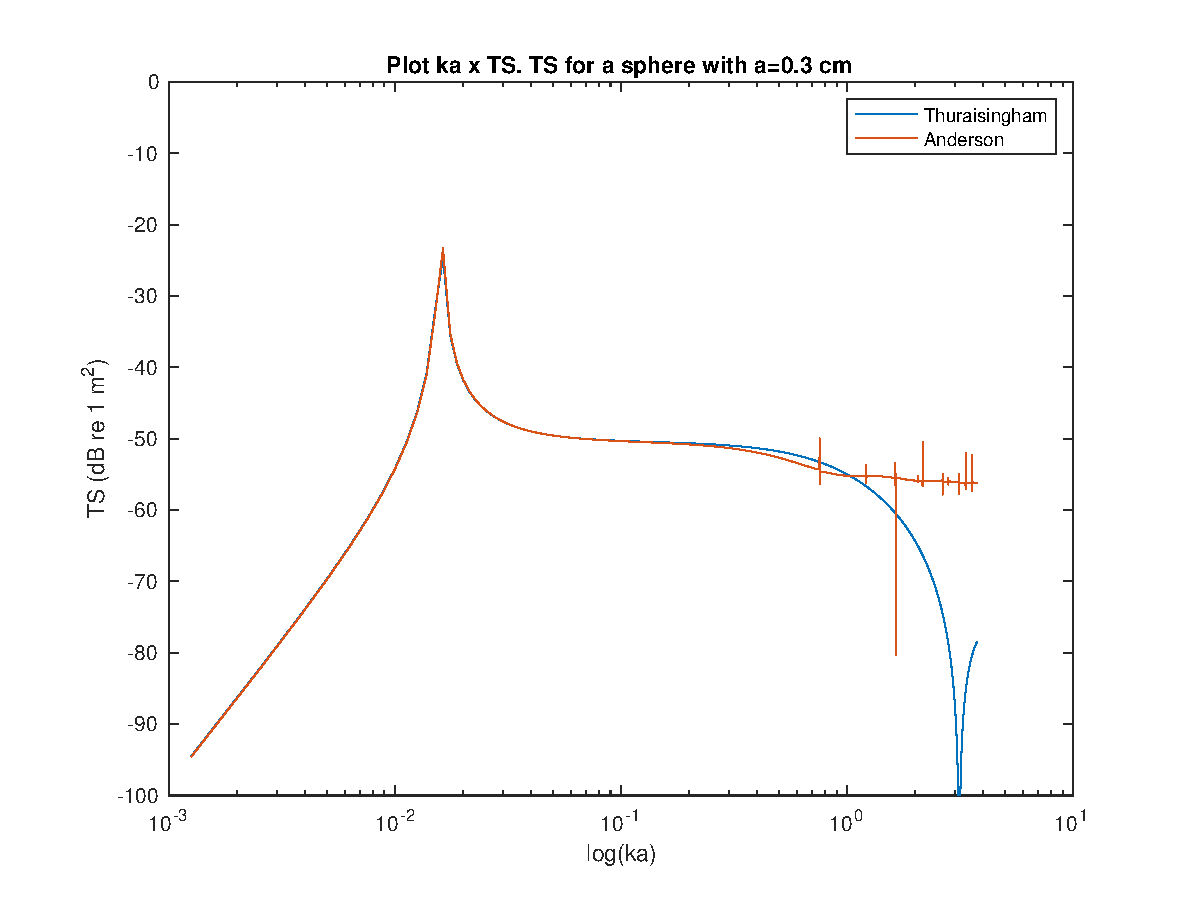
\includegraphics[width=0.7\textwidth]{thur-and-models.eps}
    \caption*{Target strength over $ka$-values for a Thuraisingham and Anderson solutions of a single bubble of radius a = 0.3 cm}
    \label{fig:thur-anderson}
\end{figure}

Figure \ref*{fig:thur-anderson} shows a plot of the single bubble target strength against  $ka << 1$, and significantly larger values $ka > 1$. The highes peak corresponds to the resonance frequency of the bubble, following smaller peaks of the modal solution might correspond to the normal modes of the bubble, which occur as a resulting oscillations. Yet it doesn't take into account the damping effect present in a bubble.


\subsection{Multiple bubble model}

For more than one bubble we can add various scenarious for bubbles' location in space, distance between each other, their dimensions, dynamics, and interactions. Those new properties pose more challenges in constructing a valid model for multiple bubbles.

Among the possible real-world applications are gas seapages underwater, bubble curtains which play role of sound attenuators.

% math assumptions and formulations

\subsubsection{Volume-scattering strength} 
In case we have more than one bubble, where we were describing it with a target strength, the volume backscattering strength should be used instead.
\[s_v = \int\sigma_{bs}n(a)\]
\[S_v = 10\log_{10}(s_v)(dB\;re\;1m^2)\]

% More bubbles are added

\subsection{Multiple scattering }

Leblond et al. paper states that for multiple discrete bubbles, we can neglect the effect of the multiple scattering \cite[]{leblond_acoustic_2014}. 
\textcolor{red}{Foldy paper equation explanation and concept of the multiple scattering}

When the signal is emitted, the scatterer removes from the wave a specific amount of flux which is equal to the its extintion cross section multiplied by flux per unit area. This amount is partially absorbed and scattered. The next step lies in adding up all the scattering from the received transmitted signal scatterer to other bubbles, then repeating the procedure in the regard of other bubbles, till all scatterers in the close enough vicinity of each other got an interaction with each other.

\begin{figure}[H]
    \centering
    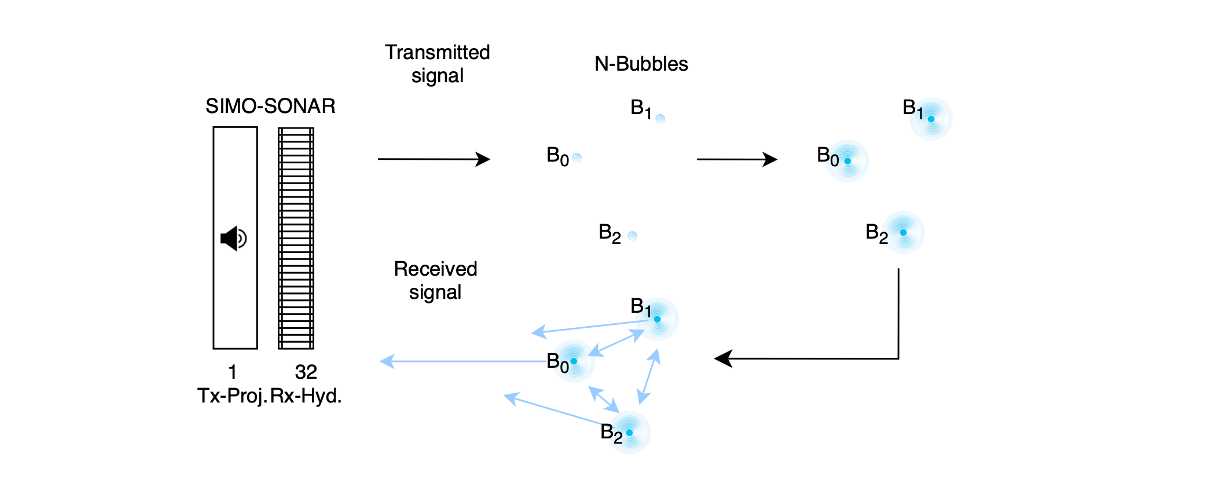
\includegraphics[width=0.7\textwidth]{multiple-scattering.png}
    \caption*{The scheme of the multiple scattering}
    \label{fig:multiple-scattering}
\end{figure}

But this concept is applicable when amount of scatterers is sufficiently small, otherwise they start interacting with each other and no longer act as a scatter independently. %source????? Foldy or Hazard?

Hazard and Cassier paper provides a mathematical point of view at the multiple scattering with a justification of the Foldy-Lax model. This model help to get an approximation of scattered waves in a deterministic as well as in a random media. Also, local error estimates for circular objects in 2D problem were obtained in the scope of results of this paper.

- Foldy, Leslie L. ‘The Multiple Scattering of Waves. I. General Theory of Isotropic Scattering by Randomly Distributed Scatterers’. Physical Review 67, no. 3–4 (1 February 1945): 107–19. https://doi.org/10.1103/PhysRev.67.107.

- Multiple Scattering of Acoustic Waves by Small Sound-Soft Obstacles in Two Dimensions: Mathematical Justification of the Foldy–Lax Model, Hazard and Cassier


\section{Reconstruction of the bubble frequency response}

It will allow demonstrating the ability to invert the model to find individual bubble contributions from compund analysis.
The following equation\ref{eqn:reconstruction_bubble} was the base of the calculations:

\begin{equation}\label{eqn:reconstruction_bubble}
    R = T \times H + N
\end{equation}
where R is a received signal, T is a transmitted signal by sonar, H is frequency response of the bubble, N is an added background noise.

\section{Signal Processing}
\subsection{Beamforming}
\begin{itemize}
    \item reconstruction of the bubble frequency response from the received signal
    \item beamforming
    \item cross-correlation, matched filtering
    \item sonar equation
\end{itemize}

A beamforming is a way of processing the received or transmitted signal, so that we can direct the directed and amplified signal from teh projector with multiple receivers or transmitters, therefore improving the SNR and eliminating unwanted interfering signals. Also, it can be referred as a spatial filtering.

Withing the scope of the work we have used beamforming in the sonar environment. A conventional beamformer in the form of the delay-and-sum was used. 
\subsection{SONAR}
\subsection{Sonar equation }
The Sonar equation is a fundamental tool in underwater acoustics used to predict the performance of sonar systems. 
The basic form of the Sonar equation is:
\begin{equation}
    SNR=SL-TL+TS-NL
\end{equation}

Where
SNR is the signal-to-noise ratio,
SL is the source level,
TL is the transmission loss,
TS is the target strength, and
NL is the noise level.

To implement the Sonar equation, one needs to calculate or estimate each of these parameters. 
Source level (SL) represents the acoustic power radiated by the sonar system, which can be determined based on the characteristics of the sonar transducer and the electrical input power. 
Transmission loss (TL) accounts for the attenuation of sound energy as it propagates through the water, considering factors such as spreading loss, absorption, and bottom and surface reflections. 
Target strength (TS) quantifies the amount of sound energy reflected or scattered by the target, which depends on its size, shape, and composition. 
Noise level (NL) encompasses all sources of ambient noise in the environment, including thermal noise, wind-generated noise, biological noise, and anthropogenic noise.



\section{Chapter Three Title}
This section will include the simulation and programming part of the work, experimental part

\subsection{Simulation of bubble response}

\subsection{Experiment of measuring bubbles}


% \begin{tabular}{l r}
%     Date Performed: & May 17, 2024 \\ % Date the experiment was performed
%     Partners: & Viktoriia \textsc{Boichenko} \\
%     Supervisor: & Christian \textsc{Kanarski} % Instructor/supervisor
% \end{tabular}


% If you need to include an abstract, uncomment the lines below
%\begin{abstract}
%	Abstract text
%\end{abstract}

%----------------------------------------------------------------------------------------
%	OBJECTIVE
%----------------------------------------------------------------------------------------

\subsection{Objective}

This laboratory project aims to connect theoretical concepts with empirical observations through the use of volume strength backscattering. The primary objective is to illustrate the practical applications of theoretical knowledge acquired during the internship and master’s thesis research. By leveraging volume strength backscattering as a key analytical tool, we will examine experimental data, providing insights into how theoretical abstractions translate into concrete experimental methodologies. This integration is designed to promote a comprehensive understanding of the reciprocal relationship between theory and practice, underscoring the significance of a multidimensional approach in scientific inquiry and engineering practice.

\begin{description}
	\item[Sonars] 

    The general principle of the projector SIMO-sonar is in the following way:  the signal is emitted with a single transducer and receiving a signal back with several receivers, which in our case were hydrophones. Also, it can be considered with another interpretation. For example, we provide a single output, and obtain multiple input data.
    
    The sonar type is the SIMO-sonar, as we needed to start with a simple model of the current research. The experiments with a MIMO-sonar can be implemented for further research therefore expanding the complexity and variability of usages of the developed model, as [this type provides an improved resolution and enhances the signal-to-noise ratio of the received signal] (http://jset.sasapublications.com/wp-content/uploads/2017/09/6702529.pdf).
    
	\item[Bubble flare] 

    A continuous column of bubbles with the different radii which is emitted with a bubble generator. Minimum bubble size that the machine could produce were 
	\item[] 
    
    %or whatever definition you want to add 
\end{description} 

\subsection{Experimental model}

The experimental setup entails an experiment of bubbles flares detection with a sonar. They were emitted in a water with a bubble generator and observed with the help of the SIMO-sonar with an ultrasound in a laboratory conditions of the water tank. 

Preliminary tests of the water tank were performed in order to identify the impulse response of the  environment, and verify the correctness of the equipment configuration as well as whether it is in a usable condition.

The primary focus of the observation was the volume strength back scattering (Vs), chosen as the key parameter for assessing the acoustic bubble response with acoustic radiation in the high-frequency range. 

\subsection{ The setup}

Our bubble experiment was conducted using a meticulously designed setup aimed at exploring the acoustic frequency response of the bubbles. The experimental arrangement included the following:
\begin{itemize}
    \item \textbf{Bubble generator}: a set of the equipment which included
    \item \textbf{Sonar} it is a projector with 32 hydrophones in an array. The distance between elements is 0.0139 m.
    \item \textbf{Laptop with a processing software KiRAT, contains an inbuilt wave generator}
    \item \textbf{Videocamera}: a mobilephone's camera was used for the experiment recordings
\end{itemize}

During the experiment different signal types (noise and chirp) and length (2 ms and 10 ms) were used for the analysis of the bubble flares. The emitted central frequency was 50 kHz with a bandwidth of 40 kHz. The sampling frequency was 192 kHz.
\begin{itemize}
    \item \textbf{Noise}: a white noise whose frequency is not dependent on the power spectral density \cite*{ainslie_principles_2010};  
    \item \textbf{Chirp}: a hyperbolic frequency modulation upward signal 
\end{itemize}


% \begin{figure}[H]
%     \includegraphics[width='0.7'\textwidth]{'setup/'}
%     \centering
%     \caption*{'caption'}
% \end{figure}


% If you have more than one objective, uncomment the below:
%\begin{description}
%	\item[First Objective] \hfill \\
%	Objective 1 text
%	\item[Second Objective] \hfill \\
%	Objective 2 text
%\end{description}
 
%----------------------------------------------------------------------------------------
%	EXPERIMENTAL DATA
%----------------------------------------------------------------------------------------

\subsection{Experimental Data}


After the pocessing the date of 23 recorded measurements, a few results as well as comparisons can be presented below. 

At the horizontal orientation samples 8 (noise, 10ms) and 11 (chirp, 10ms).

At the vertical orientation sample 19 (noise) and 23 (chirp, 10ms) are seem to be good for comparison.

\textbf{$H_{wall}$} can be extracted from the initial measurement, calculating an impulse response of the water tank and identifying the location of the walls with the sonar.

% \begin{figure}[H]
%     \includegraphics[width='0.7'\textwidth]{'experiments/anima22_2'}
%     \centering
%     \caption*{'Vertical orientation of the sonar, chirp'}
%     \label{fig:V_chirp_2ms_anima}
% \end{figure}

%----------------------------------------------------------------------------------------
%	SAMPLE CALCULATION
%----------------------------------------------------------------------------------------

\subsection{Calculations}

\begin{itemize}
    \item Vs from a single ping
    \item spectrogram in Audacity for different samples
    \item bubble localization?
    \item obtaining $H_{bubble}$, $H_{wall}$
\end{itemize}

%----------------------------------------------------------------------------------------
%	RESULTS AND CONCLUSIONS
%----------------------------------------------------------------------------------------

\subsection{Results and Conclusions}


%----------------------------------------------------------------------------------------
%	DISCUSSION
%----------------------------------------------------------------------------------------

\subsection{Discussion of Experimental Uncertainty}

% The accepted value (periodic table) is \SI{24.3}{\gram\per\mole} \autocite{Smith:2022qr}. The percentage discrepancy between the accepted value and the result obtained here is 1.3\%. Because only a single measurement was made, it is not possible to calculate an estimated standard deviation (see \textcite{Smith:2021jd}).

% The most obvious source of experimental uncertainty is the limited precision of the balance. Other potential sources of experimental uncertainty are: the reaction might not be complete; if not enough time was allowed for total oxidation, less than complete oxidation of the magnesium might have, in part, reacted with nitrogen in the air (incorrect reaction); the magnesium oxide might have absorbed water from the air, and thus weigh ``too much." Because the result obtained is close to the accepted value it is possible that some of these experimental uncertainties have fortuitously cancelled one another.



\section{Chapter Four Title}
your another content 4

\section{Conclusion}
\input{sections/conclusion}

\nocite{*}
\printbibliography[heading=bibintoc]

\begin{appendix}
% appendices : 10 pages maximum
\input{sections/appendix}
\end{appendix}

\end{document}